\section{Introduction}\label{sec:introduction}

Preserving and restoring old films is essential for safeguarding the cultural and historical heritage embedded in moving images from earlier eras~\cite{kokaram1998motion}. As physical film materials deteriorate through chemical decay, mechanical wear, and improper storage, digital restoration becomes a practical means of recovering damaged visual records~\cite{iizuka2019deepremaster}. In practice, old footage rarely exhibits a single isolated degradation. It typically combines spatially localized defects, such as scratches, dust, and blotches, with temporally varying photometric artifacts, such as brightness flicker and fading, as well as noise or grain introduced by aging and acquisition~\cite{rtn2022,wan2020bringing}. Because these degradations arise at different spatial and temporal scales, an effective degradation indicator should capture both high-frequency local anomalies and low-frequency frame-level variation, rather than relying solely on a single pixel-domain difference map.

Learning-based old film restoration (OFR) has advanced rapidly with deep low-level vision models~\cite{su2022survey,tian2020deep_denoising}. DeepRemaster~\cite{iizuka2019deepremaster} formulates spatiotemporal restoration with 3D convolutions and reference-based colorization. RTN~\cite{rtn2022} introduces bidirectional recurrent propagation with a learnable defect mask, where a pixel-domain degradation indicator gates the aggregation of propagated and current-frame features. RRTN~\cite{rrtn2024} further improves alignment with recursive transformer blocks and second-order grid propagation. MambaOFR~\cite{mao2025mambaofr} replaces heavier restoration modules with efficient Mamba-based~\cite{guo2024mambair} components and degradation-aware prompting. Despite this progress, recurrent OFR still commonly relies on a spatial-domain frame-difference signal for gating~\cite{rtn2022}. Although attractive for its simplicity, such a signal is not equally sensitive to the mixed artifacts present in old films.

Figure~\ref{fig:motivation} highlights the two cases that motivate this work. First, spatially sparse high-frequency damage, such as thin scratches and isolated dust, may affect only a small number of pixels and can therefore be diluted in a dense pixel-domain difference map. Second, brightness flicker is broad and low-frequency, often appearing as a near-uniform temporal offset that is difficult to disentangle from legitimate scene illumination changes using pixel differences alone. Treating these two regimes with the same detector can therefore yield an ambiguous gating signal for recurrent restoration.

Wavelet analysis offers a natural multi-resolution representation for separating these regimes~\cite{mallat1989theory}. The Haar discrete wavelet transform (DWT) decomposes an image into one low-frequency approximation band (LL) and three directional high-frequency detail bands (LH, HL, and HH). More broadly, wavelet coefficients have been used as localized damage evidence in signal-analysis detection settings, including continuous-wavelet-transform features coupled with sparse autoencoders~\cite{bernardini2025driveby}. Of course, wavelet coefficients are not semantic labels: motion boundaries and textured content can also activate detail bands. Even so, the decomposition provides a practical basis for OFR, because the high-frequency bands concentrate abrupt local discontinuities relevant to scratches and dust~\cite{liu2018mwcnn}, whereas the LL band preserves coarse luminance structure that is informative for flicker. This frequency separation directly motivates the LHFM/GFM design adopted in this work.

\begin{figure}[H]
\centering
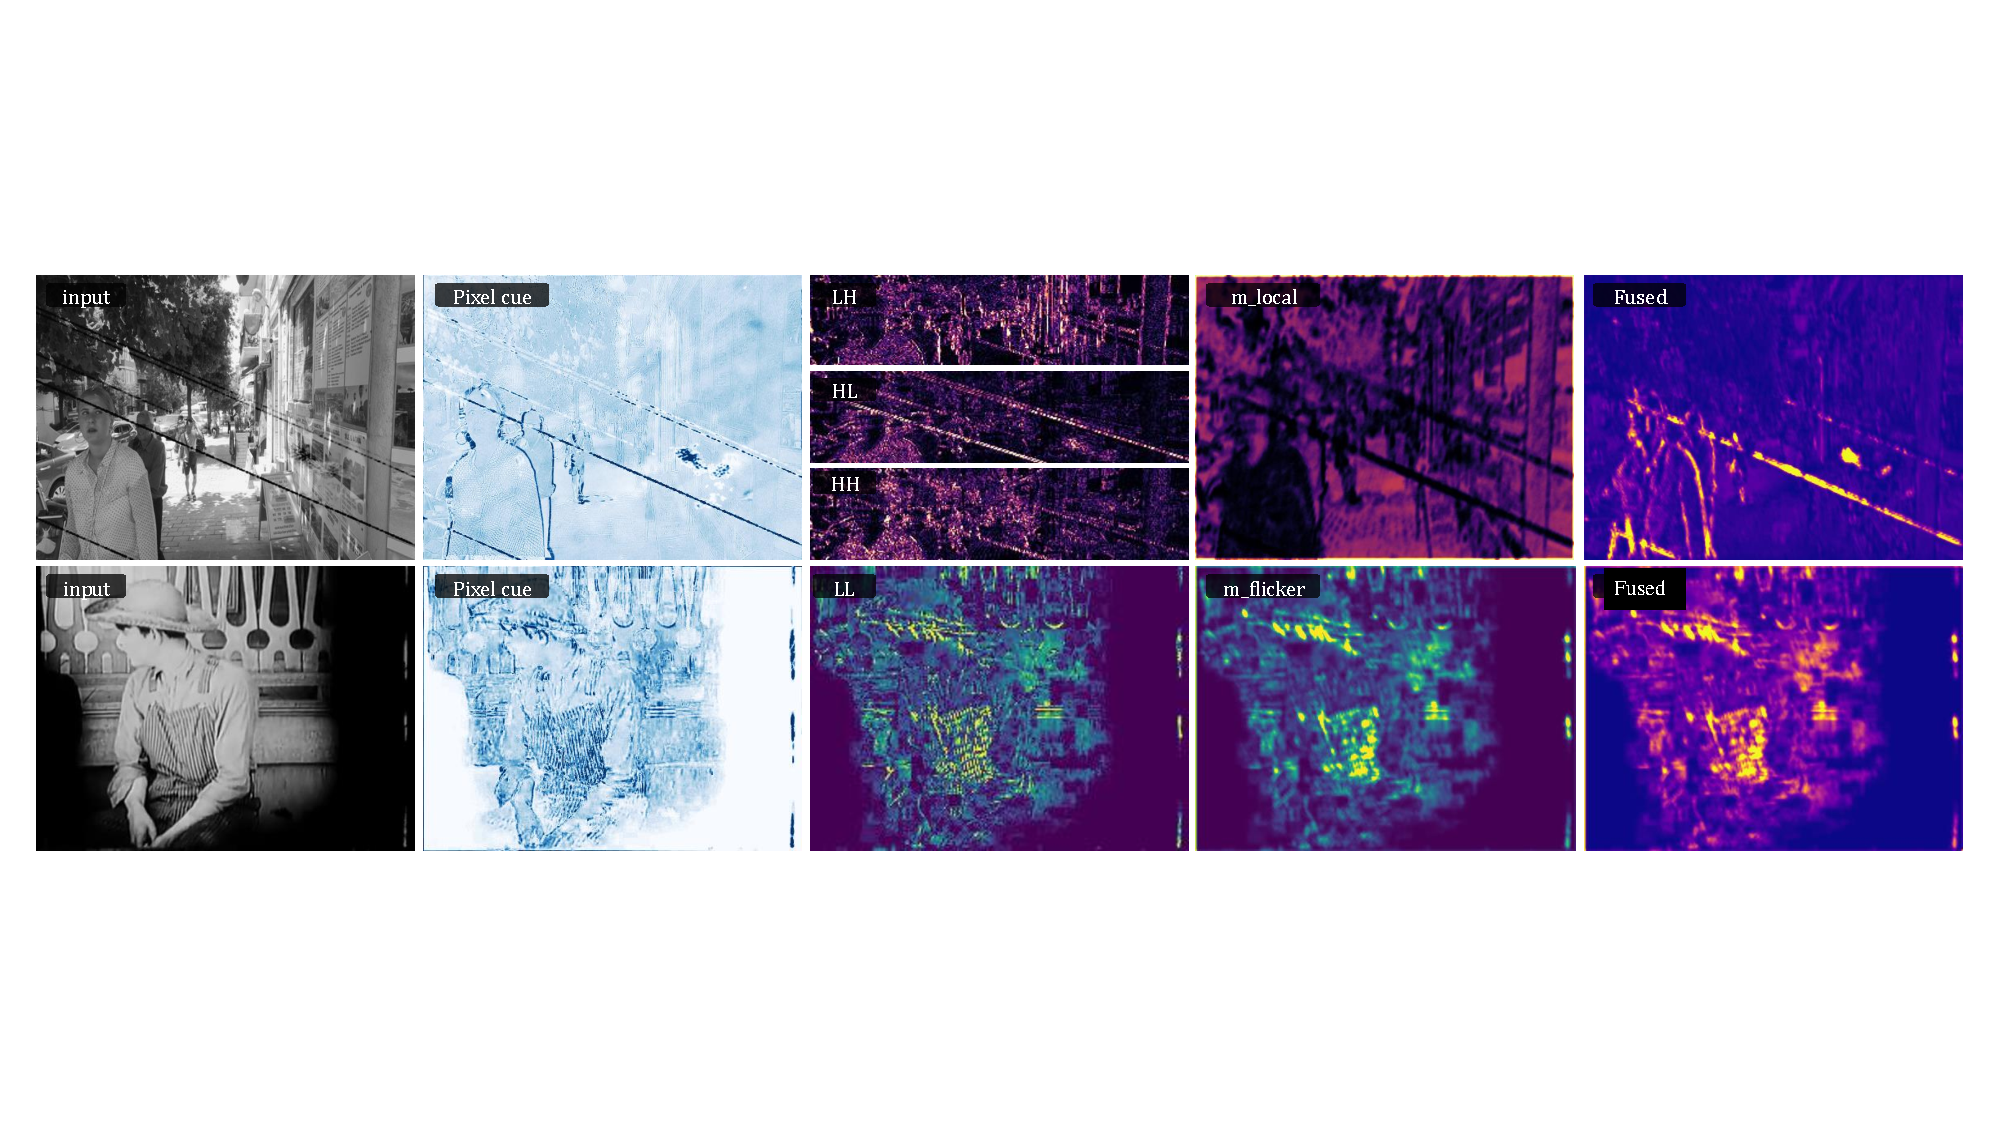
\includegraphics[width=\textwidth]{figures/Figure1.pdf}
\caption{Motivation examples for wavelet-domain degradation sensing. (a) Sparse structural damage in a synthetic validation region of interest (ROI) produces clearer Haar detail-band responses (LH/HL/HH) than the warped pixel-domain cue. (b) Brightness flicker in a real triplet from the Synthetic and Real-World Old Video (SRWOV) benchmark is emphasized by the LL temporal response and carried into the fused WaveletMask indicator. The branch-mask column reports $m_{\mathrm{local}}$ in (a) and $m_{\mathrm{flicker}}$ in (b). Except for the fixed-scale pixel cue, response and mask panels are display-normalized for visualization. The panels are qualitative motivation examples and are not used as quantitative evidence.\label{fig:motivation}}
\end{figure}

Building on this motivation, we propose \textbf{WaveletMask}, a wavelet-domain degradation detection framework for recurrent OFR. The Local High-Frequency Mask Module (LHFM; Section~\ref{subsec:local}) applies geometric-mean differencing to the Haar detail sub-bands to emphasize transient local damage. The Global Flicker Mask Module (GFM; Section~\ref{subsec:flicker}) applies a minimum-difference temporal criterion to the LL sub-band to emphasize frame-level brightness changes. The two branch masks are then combined by an element-wise maximum to form the wavelet-domain gate used for recurrent aggregation. We also evaluate learned pixel-wise fusion with the original RTN spatial indicator as an ablation. However, it is not included in the proposed model because, under the tested training recipe, it underperforms the wavelet-only gate (Table~\ref{tab:fusion_comparison}). The overall pipeline is shown in Figure~\ref{fig:pipeline}, and the two branches are detailed in Figures~\ref{fig:lhfm} and~\ref{fig:gfm}.

The main contributions are as follows:
\begin{enumerate}
    \item \textbf{WaveletMask: frequency-aware gating for recurrent OFR.} We formulate degradation sensing in the Haar wavelet domain and replace a single pixel-domain difference gate with a two-branch design that separately models high-frequency local damage and low-frequency flicker cues.

    \item \textbf{LHFM for transient structural defects.} LHFM applies geometric-mean differencing to the LH, HL, and HH sub-bands across three consecutive frames, emphasizing frame-specific scratches, dust, and other local defects while suppressing responses from persistent edges and one-sided temporal changes.

    \item \textbf{GFM for frame-level brightness instability.} GFM applies a minimum-difference criterion in the LL sub-band to detect current-frame brightness deviations relative to both temporal neighbors, yielding a dedicated cue for low-frequency flicker.

    \item \textbf{A diagnostic evaluation framework for frequency-domain degradation masks.} Under the SRWOV protocol, we establish a diagnostic evaluation framework that combines a unified re-training benchmark over ten methods with a strict paired statistical analysis against the RTN, and analyzes mask behavior through multi-seed reproducibility tests, paired clip-level significance analysis, artifact-stratified and failure-mode probes, fusion and wavelet-family ablations, and runtime measurement.
\end{enumerate}

The remainder of the paper is organized as follows. Section~\ref{sec:related_work} reviews related work. Section~\ref{sec:method} describes WaveletMask. Section~\ref{sec:results} presents synthetic, real-world, ablation, and complexity results. Section~\ref{sec:discussion} discusses interpretation, failure modes, and current limitations, including broader real-world variation and motion-related failure cases. Section~\ref{sec:conclusions} concludes the paper.
